\section{Auswertung}
\label{sec:Auswertung}

% Tabellen und Plot zu E1, erste Stange
Die Biegung $D(x)$ an den Stellen $x$ mit und ohne Gewicht
ist für den ersten Stab in Tabelle 1 zu sehen. Die Biegung ist %T1
jeweils in $\si{\mm}$ angegeben.
Die horizontale Länge $x$ ist in $\si{\cm}$ angegeben.
\begin{table}\caption{}
\label{}
\centering
\sisetup{round-mode = places, round-precision=2, round-integer-to-decimal=true}
\begin{tabular}{S[]S[]S[]} 
\toprule
{$D(x)/\si{\milli\meter}$ ohne Gewicht} & {$D(x)/\si{\milli\meter}$ mit Gewicht} & {$x/\si{\centi\meter}$}\\
\midrule
0.98 & 1.1 & 3.0\\
1.04 & 1.1 & 5.0\\
1.11 & 1.17 & 8.0\\
1.16 & 1.17 & 11.0\\
1.12 & 1.18 & 14.0\\
1.12 & 1.19 & 17.0\\
1.1 & 1.19 & 20.0\\
1.03 & 1.21 & 23.0\\
0.93 & 1.23 & 26.0\\
0.8 & 1.24 & 29.0\\
0.68 & 1.25 & 32.0\\
0.58 & 1.25 & 35.0\\
0.4 & 1.25 & 38.0\\
0.2 & 1.26 & 41.0\\
0.08 & 1.26 & 44.0\\
-0.1 & 1.26 & 47.0\\
-0.38 & 1.26 & 49.0\\
\bottomrule
\end{tabular}\end{table}

Die Differenz \eqref{eqn:} der beiden Biegungen aus Tabelle 1 %eqn:?
und $Lx^2-\frac{x^3}{3}$ sind in Tabelle 2 dargestellt. %T2
\begin{table}\caption{}
\label{}
\centering
\sisetup{round-mode = places, round-precision=2, round-integer-to-decimal=true}
\begin{tabular}{S[]S[]} 
\toprule
{$D(x)/m$ Differenz} & {$Lx^2-x^3/3 /m^3$}\\
\midrule
0.00012000000000000011 & 0.0004751999999999999\\
6.0000000000000056e-05 & 0.0013033333333333334\\
5.999999999999983e-05 & 0.003272533333333333\\
1.000000000000001e-05 & 0.006066133333333332\\
5.999999999999983e-05 & 0.009630133333333332\\
6.999999999999984e-05 & 0.013910533333333334\\
8.999999999999986e-05 & 0.018853333333333333\\
0.00017999999999999993 & 0.024404533333333332\\
0.0002999999999999999 & 0.03051013333333333\\
0.00043999999999999996 & 0.03711613333333332\\
0.00057 & 0.04416853333333332\\
0.00067 & 0.05161333333333332\\
0.00085 & 0.05939653333333332\\
0.00106 & 0.06746413333333331\\
0.0011799999999999998 & 0.07576213333333331\\
0.00136 & 0.08423653333333331\\
0.0016400000000000002 & 0.08995746666666665\\
\bottomrule
\end{tabular}\end{table}

Auf diese Weise lässt sich mit Hilfe des Graphen %Plot1
der Elastizitätsmodul durch die Steigung bestimmen. %eqn:E
\begin{figure}
  \centering
  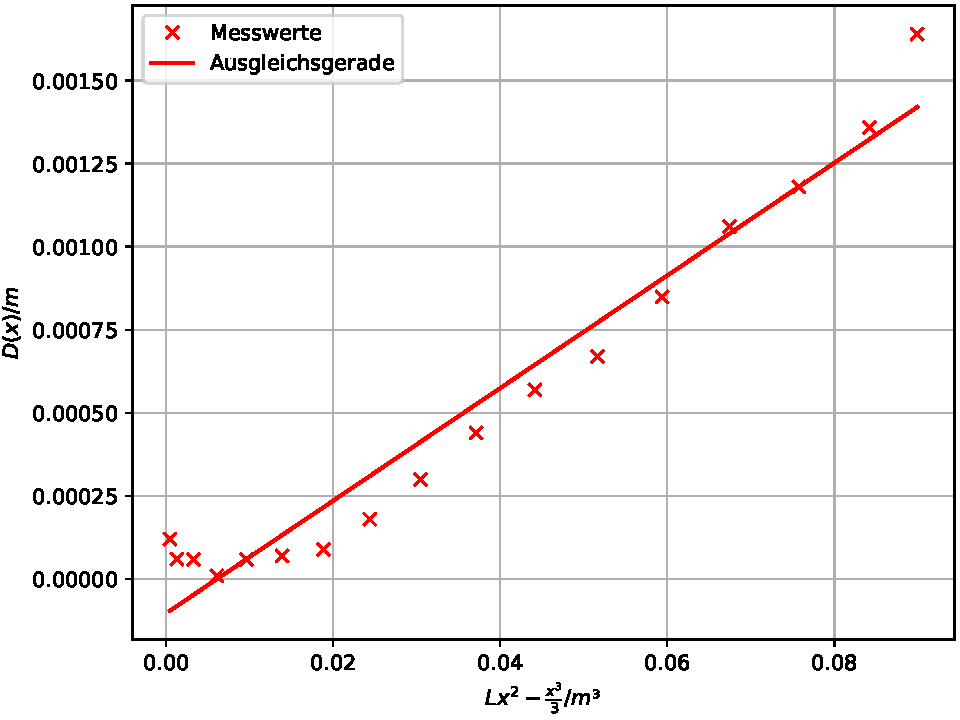
\includegraphics[width=12cm, height=9cm]{./plots/Stange1.pdf}
  \caption{Plot.}
  \label{fig:plot}
\end{figure}
Die Steigung ergibt sich mit %eqn:m
zu $m = \SI{1.694e-2}{}$. Damit ist der Elastizitätsmodul mit %eqn:E, Steigung SI
$E = \SI[per-mode=fraction]{4.590e11}{\Newton\per\square\metre}$. %?

% Tabellen und Plot zu E2, zweite Stange
\begin{table}\caption{}Vertikaler Abstand der Stange zur Messuhr mit und ohne Gewicht,
Abstand der Messuhr vom Ursprung auf der horizontalen Achse
\label{table: D2}
\centering
\sisetup{round-mode = places, round-precision=2, round-integer-to-decimal=true}
\begin{tabular}{S[]S[]S[]} 
\toprule
{$D(x)/\si{\milli\meter}$ ohne Gewicht} & {$D(x)/\si{\milli\meter}$ mit Gewicht} & {$x/\si{\centi\meter}$}\\
\midrule
0.87 & 0.79 & 3.0\\
0.91 & 0.77 & 5.0\\
0.98 & 0.68 & 8.0\\
1.01 & 0.5 & 11.0\\
1.03 & 0.27 & 14.0\\
1.03 & -0.05 & 17.0\\
1.04 & -0.42 & 20.0\\
0.96 & -1.3 & 26.0\\
0.88 & -1.83 & 29.0\\
0.82 & -2.42 & 32.0\\
0.69 & -3.13 & 35.0\\
0.55 & -3.71 & 38.0\\
0.36 & -4.41 & 41.0\\
0.1 & -5.23 & 44.0\\
-0.15 & -6.16 & 47.0\\
-0.33 & -6.56 & 49.0\\
\bottomrule
\end{tabular}\end{table}


\begin{table}\caption{}
\label{}
\centering
\sisetup{round-mode = places, round-precision=2, round-integer-to-decimal=true}
\begin{tabular}{S[]S[]} 
\toprule
{D(x) in m} & {x in m³}\\
\midrule
7.999999999999997e-05 & 0.0004518\\
0.00014000000000000001 & 0.0012383333333333337\\
0.0002999999999999999 & 0.0031061333333333337\\
0.00051 & 0.005751533333333333\\
0.00076 & 0.009120533333333333\\
0.00108 & 0.013159133333333335\\
0.00146 & 0.017813333333333337\\
0.00226 & 0.028752533333333333\\
0.00271 & 0.03492953333333333\\
0.00324 & 0.041506133333333334\\
0.00382 & 0.04842833333333334\\
0.00426 & 0.05564213333333334\\
0.004770000000000001 & 0.06309353333333333\\
0.00533 & 0.07072853333333333\\
0.00601 & 0.07849313333333334\\
0.006229999999999999 & 0.08371486666666667\\
\bottomrule
\end{tabular}\end{table}

\begin{figure}
  \centering
  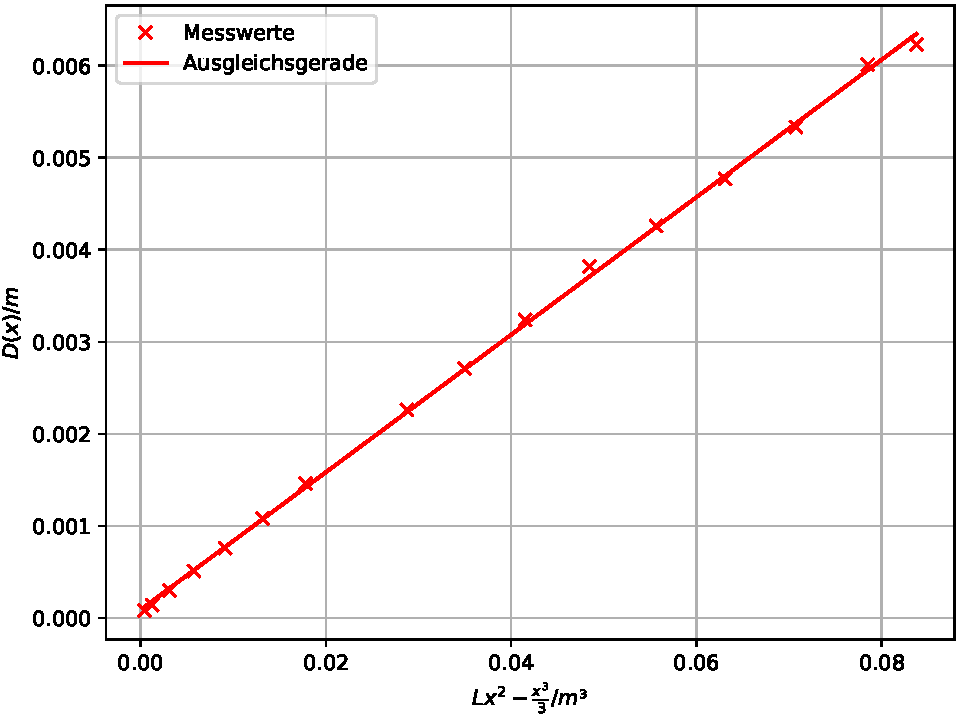
\includegraphics[width=12cm, height=9cm]{./plots/Stange2.pdf}
  \caption{Plot.}
  \label{fig:plot}
\end{figure}

% Tabellen und Plot zu E3a, dritte Stange
\begin{table}\caption{}
\label{}
\centering
\sisetup{round-mode = places, round-precision=2, round-integer-to-decimal=true}
\begin{tabular}{S[]S[]S[]} 
\toprule
{D(x)ohne} & {D(x)mit} & {x}\\
\midrule
0.75 & 0.71 & 3.0\\
0.79 & 0.72 & 5.0\\
0.82 & 0.72 & 8.0\\
0.83 & 0.7 & 11.0\\
0.8 & 0.6 & 14.0\\
0.74 & 0.49 & 17.0\\
0.66 & 0.34 & 20.0\\
0.55 & 0.19 & 23.0\\
0.66 & 0.34 & 20.0\\
0.55 & 0.19 & 23.0\\
0.45 & 0.05 & 26.0\\
\bottomrule
\end{tabular}\end{table}

\begin{table}\caption{}
\label{}
\centering
\sisetup{round-mode = places, round-precision=5, round-integer-to-decimal=true}
\begin{tabular}{S[]S[]} 
\toprule
{$D(x)/m$ Differenz} & {$3L^2x-4x^3 /m^3$}\\
\midrule
4.000000000000004e-05 & 0.02821689000000001\\
7.000000000000006e-05 & 0.04670815000000002\\
9.999999999999998e-05 & 0.07348504000000003\\
0.00013000000000000002 & 0.09853393000000003\\
0.00020000000000000006 & 0.12120682000000006\\
0.00025 & 0.14085571000000005\\
0.00032 & 0.15683260000000007\\
0.00036 & 0.16848949000000008\\
0.00032 & 0.15683260000000007\\
0.00036 & 0.16848949000000008\\
0.0004 & 0.17517838000000008\\
\bottomrule
\end{tabular}\end{table}


\begin{figure}
  \centering
  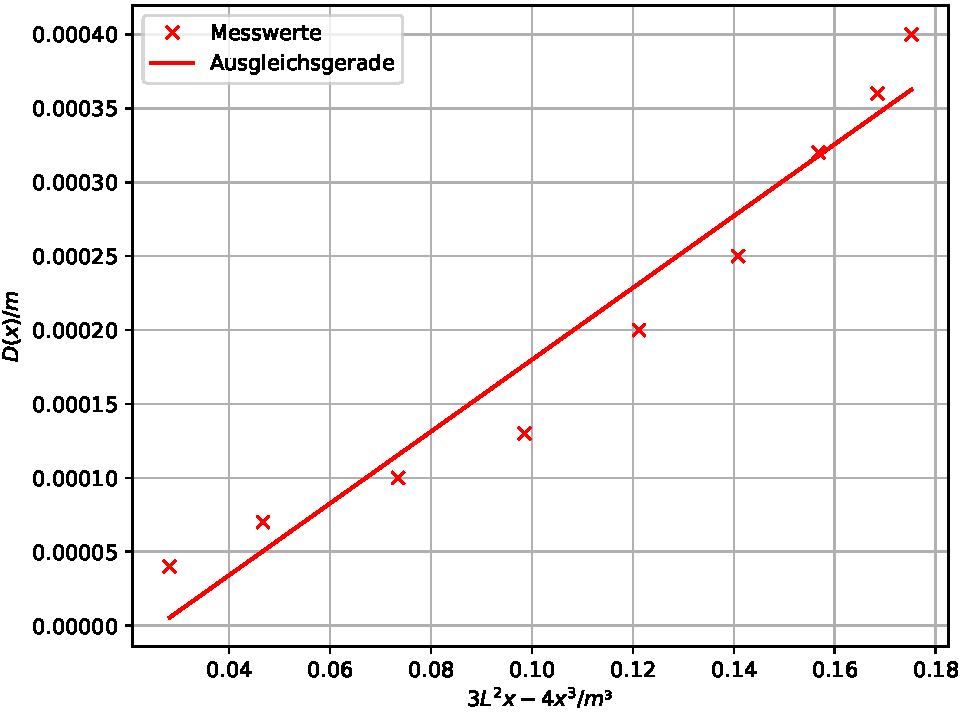
\includegraphics[width=12cm, height=9cm]{./plots/Stange3a.pdf}
  \caption{Plot.}
  \label{fig:plot}
\end{figure}

% Tabellen und Plot zu E3b, dritte Stange
\begin{table}\caption{}
\label{}
\centering
\sisetup{round-mode = places, round-precision=2, round-integer-to-decimal=true}
\begin{tabular}{S[]S[]S[]} 
\toprule
{$D(x)/mm$ ohne Gewicht} & {$D(x)/mm$ mit Gewicht} & {$x/cm$}\\
\midrule
-1.01 & -1.75 & 29.0\\
-0.97 & -1.79 & 32.0\\
-1.08 & -1.89 & 35.0\\
-1.16 & -1.98 & 38.0\\
-1.35 & -2.08 & 41.0\\
-1.48 & -2.13 & 44.0\\
-1.58 & -2.15 & 47.0\\
-1.67 & -2.12 & 50.0\\
-1.76 & -2.06 & 53.0\\
\bottomrule
\end{tabular}\end{table}

\begin{table}\caption{}
\label{}
\centering
\sisetup{round-mode = places, round-precision=2, round-integer-to-decimal=true}
\begin{tabular}{S[]S[]} 
\toprule
{$D(x)/\si{\meter}$ Differenz} & {$4x^3-12Lx^2+9L^2x-L^3 /\si{\cubic\meter}$}\\
\midrule
0.00074 & 0.17625812900000004\\
0.0008200000000000001 & 0.1715531990000002\\
0.0008099999999999998 & 0.16164266900000013\\
0.0008200000000000001 & 0.147174539\\
0.00073 & 0.12879680900000012\\
0.0006499999999999999 & 0.10715747900000006\\
0.0005699999999999999 & 0.08290454900000022\\
0.0004500000000000002 & 0.05668601900000003\\
0.00030000000000000003 & 0.029149888999999707\\
\bottomrule
\end{tabular}\end{table}

\begin{figure}
  \centering
  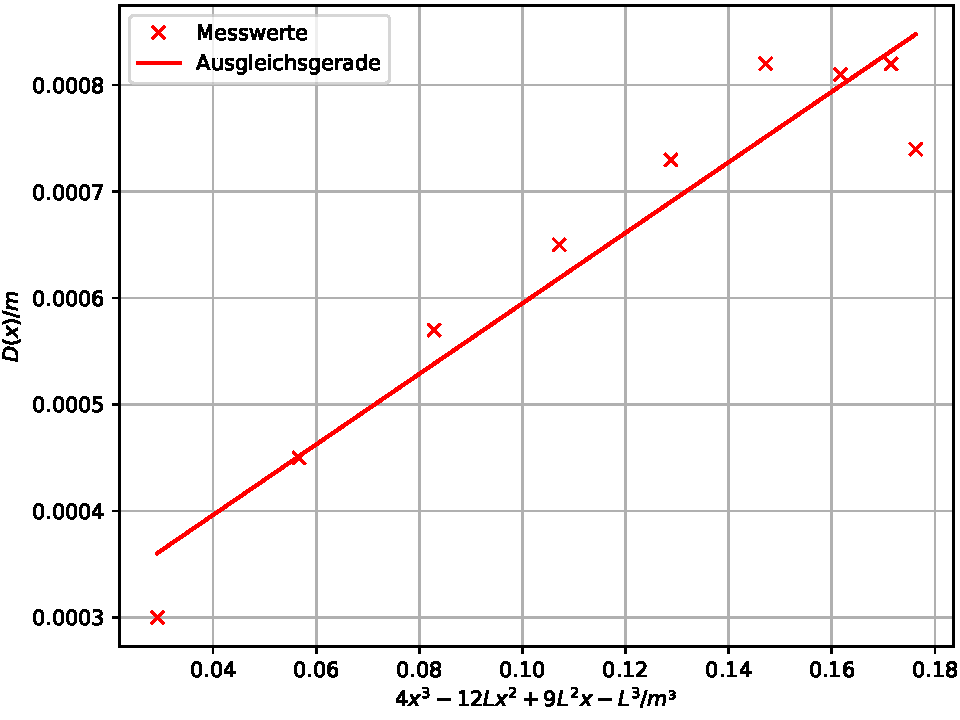
\includegraphics[width=12cm, height=9cm]{./plots/Stange3b.pdf}
  \caption{Plot.}
  \label{fig:plot}
\end{figure}
